\chapter{From the derivations to the reported results}
\label{worked:chapter}

The preceding chapters establish relationships among population quantities. A figure or fitted estimate additionally specifies numerical inputs and a calculation. This chapter makes that connection explicit. It develops the substitutions behind the main figures and visual examples, then explains what is computed from simulated observations. The source paths in Appendix~\ref{coverage:chapter} locate the complete calculations, including their random seeds and saved results.

\section{What can be derived and what must be computed?}
\label{worked:status}

For a stated Gaussian population and an exact quadratic target, the component formulas are identities. Their numerical evaluation is a substitution into a proved expression. The population parameters can instead be used to generate a finite random sample. A discrepancy measured in that sample is a random numerical result; its particular value depends on the sample, although its definition follows from the theory. Finally, an estimate obtained by maximising a likelihood and its bootstrap interval depend on the observed data, optimisation and refitting procedure. A proof of the likelihood formula does not specify the maximiser without performing that calculation.

These distinctions determine what reproduction means. An analytical result is reproduced by following its proof under its assumptions. A generated example is reproduced by using its recorded parameters and random stream. A fitted result is reproduced by fitting the same observation model to the same observations and repeating its stated uncertainty calculation. The repository supplies all three forms of material.

\section{Constructing the conditional fitness curve}
\label{worked:main1}

Main Figure 1 uses $Z=A+E$, independent $E\sim N(0,0.49)$, optimum $\theta=1$ and phenotype-fitness width $\omega=0.6$. The population has mean breeding value zero and breeding-value variance $G=0.49$. The environmental calculation in Chapter~\ref{conditioning:chapter} gives
\begin{align}
 W_A(a)
 &=\sqrt{\frac{0.36}{0.36+0.49}}\,
    \exp\!\left[-\frac{(a-1)^2}{2(0.36+0.49)}\right],\\
 \ell_A(a)
 &=\frac12\log\frac{0.36}{0.85}-\frac{(a-1)^2}{1.70}.
\end{align}
The overall fitness multiplier is one in this example. Differentiating before substituting the reference mean gives
\[
 \ell_A'(a)=\frac{1-a}{0.85},
 \qquad
 \ell_A''(a)=-\frac{1}{0.85}.
\]
Consequently $b=20/17=1.1764705882$ and $H=-20/17$. The breeding-value variance determines how often different parts of this curve occur; it does not enter this environmental averaging integral. In contrast, the environmental variance changes the curve itself.

The points in this construction are phenotype-dependent fitness values assigned after drawing environmental deviations. They are not Poisson offspring-count observations. Repeating the environmental average numerically checks the integration, with a recorded maximum absolute discrepancy of about $0.001817$ over the tested values. That discrepancy is a Monte Carlo result, not an additional term in $W_A$.

\paragraph{Biological interpretation.}
Individuals sharing a breeding value can experience different environments and receive different reproductive weights. The conditional mean averages those differences. The curve relevant to breeding values therefore has a different curvature from the original phenotype-fitness function.

\section{Checking a population identity with finite samples}
\label{worked:main2}

Main Figure 2 generates 360 combinations of $\vect b$, $\mat H$ and $\mat G$ in dimensions 2, 4 and 8. For each combination it draws 20,000 Gaussian breeding-value vectors. The exact population value is
\[
 A_{\rm theory}
 =\frac{\vect b^{\mathsf T}\mat G\vect b}
 {\vect b^{\mathsf T}\mat G\vect b+
   \tfrac12\tr(\mat H\mat G\mat H\mat G)}.
\]
For a particular generated sample, form $L_i=\vect b^{\mathsf T}\vect X_i$ and
$Y_i=L_i+\{\vect X_i^{\mathsf T}\mat H\vect X_i-\tr(\mat H\mat G)\}/2$.
The sample comparison is
\begin{equation}
 r^2=
 \frac{\{\sum_i(L_i-\bar L)(Y_i-\bar Y)\}^2}
 {\sum_i(L_i-\bar L)^2\sum_i(Y_i-\bar Y)^2}.
 \label{worked:sample_r2}
\end{equation}
Sample centring remains necessary: a finite sample from a centred population need not have sample mean zero. The constant used to centre the quadratic term does not change a correlation.

For each parameter combination the script records $|A_{\rm theory}-r^2|$. Across the 360 cases, the saved median is $0.0023672601$, the 95th percentile is $0.0103264192$, and the maximum is $0.0252707809$. Chapter~\ref{gaussian:chapter} proves the population identity; these discrepancies measure finite-sample agreement with it. The seed $20260905$ and the original sequence of random draws determine the recorded values.

\section{Contracting covariance without changing the surface}
\label{worked:main3}

The fixed-surface comparison uses
\[
 \mat G_0=
 \begin{pmatrix}1&0.3\\0.3&0.6\end{pmatrix},
 \qquad
 \vect b=\begin{pmatrix}0.75\\0.30\end{pmatrix},
 \qquad \mat H=-0.8\mat I .
\]
First perform the matrix--vector multiplication:
\[
 \mat G_0\vect b
 =\begin{pmatrix}0.75+0.09\\0.225+0.18\end{pmatrix}
 =\begin{pmatrix}0.84\\0.405\end{pmatrix}.
\]
The linear variance is therefore
$0.75(0.84)+0.30(0.405)=0.7515$. Next,
\[
 \mat G_0^2=
 \begin{pmatrix}1.09&0.48\\0.48&0.45\end{pmatrix},
 \qquad
 \Vquad=\frac{0.8^2}{2}(1.09+0.45)=0.4928.
\]
The share is $0.7515/(0.7515+0.4928)=0.6039540304$.

For the narrower population $\mat G_1=0.11\mat G_0$, Chapter~\ref{geometry:chapter} gives
\begin{align}
 \Vlin(\mat G_1)&=0.11(0.7515)=0.082665,\\
 \Vquad(\mat G_1)&=0.11^2(0.4928)=0.00596288,\\
 \Ag(\mat G_1)&=\frac{0.082665}{0.082665+0.00596288}
              =0.9327200425.
\end{align}
Both absolute variances decrease. Their different scaling rates increase the fraction contributed by the linear term. This is the calculation behind Main Figure 3, not a change in the curvature or the population mean.

\section{Following the specified covariance trajectory}
\label{worked:main4}

Main Figure 4 takes four traits with $\mat G_t=g_t\mat I$, $\mat B=\mat I$,
$\bGamma=0.3\mat I$ and $\rho=0.9$. The scalar recursion becomes
\[
 g_{t+1}=0.1+0.9\frac{g_t}{1+0.3g_t},\qquad g_0=4.
\]
Its positive fixed point solves
$0.3(g^*)^2+0.07g^*-0.1=0$, giving
\[
 g^*=\frac{-0.07+\sqrt{0.07^2+0.12}}{0.6}
     =0.4723532349.
\]
The contraction result in Chapter~\ref{inheritance:chapter} explains why iterating from $g_0=4$ approaches this value. It does not specify the directional gradient. The figure separately prescribes its norm:
\[
 \norm{\vect b_t}=
 \begin{cases}
 1,&0\leq t\leq40,\\
 \exp\{-0.06(t-40)\},&40<t\leq100.
 \end{cases}
\]
For each generation,
\begin{equation}
 \Vlin(t)=g_t\norm{\vect b_t}^2,\qquad
 \Vquad(t)=\frac{4}{2}(0.3)^2g_t^2=0.18g_t^2.
 \label{worked:trajectory_components}
\end{equation}
Thus the initial components are 4 and 2.88 and the initial share is
$4/6.88=0.5813953488$. At generation 40 the iterated variance is
$0.4723535595$, giving components $0.4723535595$ and $0.0401612193$ and share
$0.9216389049$. At generation 100 the prescribed gradient norm is
$e^{-3.6}$, and substitution into Equation~\eqref{worked:trajectory_components}
gives share $0.0087044928$.

\paragraph{Biological interpretation.}
The first phase illustrates how reproduction and stabilising selection jointly change covariance under the stated closure while the gradient is maintained. The later decrease in the share follows from the imposed decline in the gradient. It is not a prediction of a moving population mean, which this covariance recursion does not calculate.

\section{One trait: broad, narrow and centred at the peak}
\label{worked:one_trait}

Appendix Figure A1 and the one-trait tutorial use one curve,
$\ell_A(a)=a-a^2/2$. Let $A\sim N(m,v)$ and write $x=a-m$. Expanding the actual polynomial, without a remainder, yields
\[
 \ell_A(m+x)=m-\frac{m^2}{2}+(1-m)x-\frac{x^2}{2}.
\]
Its local slope is $b=1-m$ and its curvature is $H=-1$. The population-fitted line includes the expected quadratic contribution:
\[
 \widehat\ell_1(m+x)
 =m-\frac{m^2}{2}-\frac v2+(1-m)x.
\]
The tangent omits $-v/2$ and therefore differs in intercept. The component calculation gives
\[
 \Vlin=(1-m)^2v,\qquad
 \Vquad=\frac{v^2}{2}.
\]
For $v>0$, their ratio is
$\Ag=(1-m)^2/\{(1-m)^2+v/2\}$.

\begin{center}
\begin{tabular}{@{}lrrrrr@{}}
\toprule Population & $m$ & $v$ & $\Vlin$ & $\Vquad$ & $\Ag$\\
\midrule
Broad &0&1&1&0.5&$2/3$\\
Narrow, same mean &0&0.1&0.1&0.005&$20/21$\\
Narrow, at the peak &1&0.1&0&0.005&0\\
\bottomrule
\end{tabular}
\end{center}

\begin{figure}[tbp]
\centering
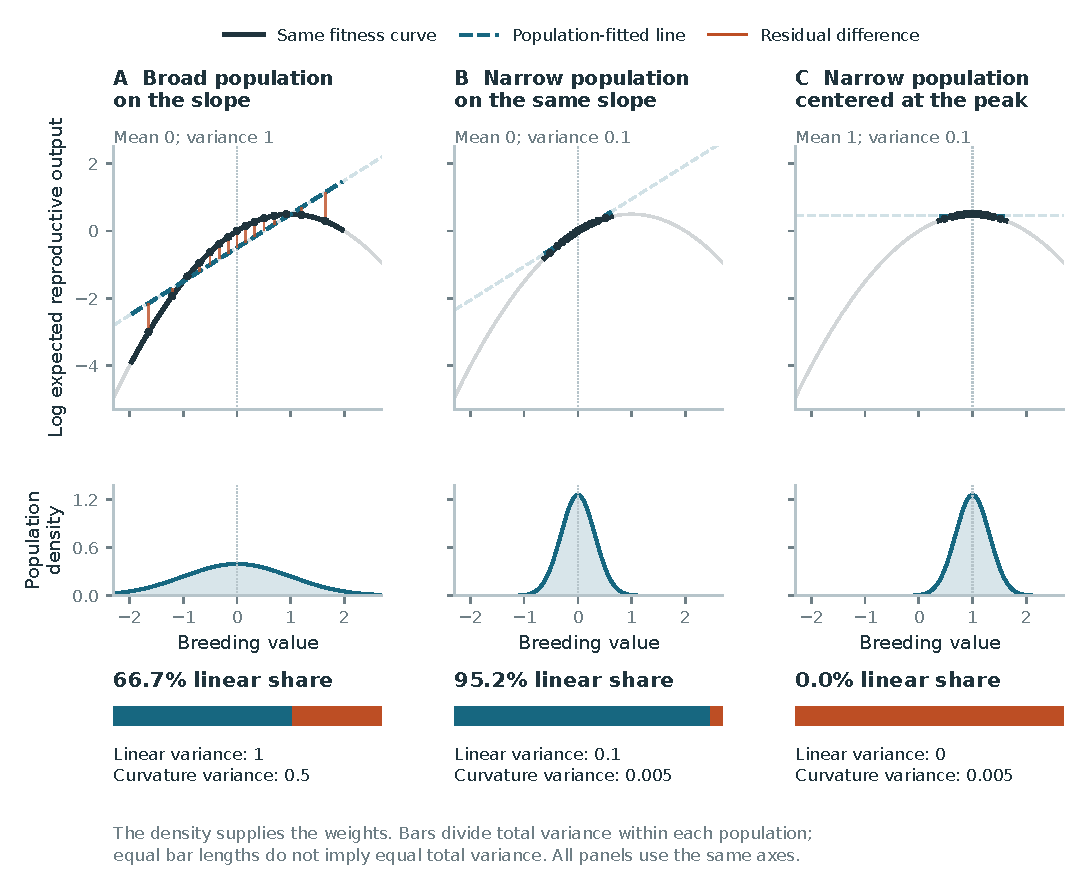
\includegraphics[width=\textwidth]{../one_trait_visual/figures/one_trait_additive_channel.pdf}
\caption{The curve is the same in all three populations. Population variance changes the weights assigned to its values; moving the mean to the peak also changes the local slope. The displayed densities are separate from the fitness scale. All values in the table are population calculations, not estimates from the plotted points.}
\label{worked:fig_one_trait}
\end{figure}

\paragraph{Biological interpretation.}
A narrow population has a large linear share in the second case because its mean is on the slope. Narrowness by itself does not give a large share: at the peak the first-order component vanishes while curvature still produces variation.

\section{Rotating the population on a fixed two-trait surface}
\label{worked:rotation}

The geometry example takes $\bGamma=0.8\mat I$ and an optimum whose original coordinates are $(0.9375,0.375)^{\mathsf T}$. An orthonormal coordinate change places the direction towards the optimum along the first axis. This preliminary relabelling does not change any variance component. The mean remains zero and the gradient is $(g,0)^{\mathsf T}$, where
\[
 g^2=(0.8)^2(0.9375^2+0.375^2)=0.6525.
\]
Now physically rotate the covariance, keeping the fitness surface and trait axes fixed:
\[
 \mat G_\varphi=\mat R_\varphi
 \begin{pmatrix}0.20&0\\0&0.005\end{pmatrix}
 \mat R_\varphi^{\mathsf T},\qquad
 \mat R_\varphi=
 \begin{pmatrix}\cos\varphi&-\sin\varphi\\
                 \sin\varphi&\cos\varphi\end{pmatrix}.
\]
Matrix multiplication gives
$G_{\varphi,11}=0.20\cos^2\varphi+0.005\sin^2\varphi$. Since only the first gradient coordinate is nonzero,
\begin{align}
 \Vlin(\varphi)&=0.6525\{0.20\cos^2\varphi+0.005\sin^2\varphi\},\\
 \Vquad(\varphi)&=\frac{0.8^2}{2}\tr(\mat G_\varphi^2)
 =\frac{0.8^2}{2}(0.20^2+0.005^2)=0.012808.
\end{align}
The second equality follows because rotation preserves the covariance eigenvalues, and the curvature is isotropic in this example. It need not hold for arbitrary curvature.

\begin{center}
\begin{tabular}{@{}lrrr@{}}
\toprule Rotation & $\Vlin$ & $\Vquad$ & $\Ag$\\
\midrule
$0^\circ$ &0.1305&0.012808&0.910626\\
$45^\circ$&0.06688125&0.012808&0.839276\\
$90^\circ$&0.0032625&0.012808&0.203012\\
\bottomrule
\end{tabular}
\end{center}
At $90^\circ$, the long axis is perpendicular to the gradient, but variance $0.005$ remains in the gradient direction. A section along the long axis therefore has zero first-order slope even though the full population has a positive linear component. A one-dimensional slice cannot replace the full two-trait calculation.

There is another angle in the teaching figures, defined between centred fitness functions under the inner product $\langle f,h\rangle=\E[fh]$. If both the linear component and total variance are positive, let $\psi$ be the angle between $L$ and $L+Q_c$. Orthogonality gives
\[
 \cos\psi
 =\frac{\E[L(L+Q_c)]}
 {\sqrt{\E[L^2]}\sqrt{\E[(L+Q_c)^2]}}
 =\sqrt{\frac{\Vlin}{\Vlin+\Vquad}},
 \qquad \Ag=\cos^2\psi.
\]
This angle is between functions, with the population supplying their inner product. It is not the physical rotation $\varphi$ of the covariance ellipse. When $L$ is the zero function, its ordinary angle is undefined; a drawn $90^\circ$ triangle then represents a limit.

\subsection{The same share from different population changes}
\label{worked:comparison}

The four geometry comparison cases alter covariance scale $s$ and the distance to the optimum by a factor $d$. With isotropic fixed curvature and the original direction to the optimum retained, the new gradient is $d\vect b_0$ and the new covariance is $s\mat G_0$. Hence
\[
 \Vlin(s,d)=sd^2L_0,\qquad
 \Vquad(s,d)=s^2Q_0,\qquad
 \Ag(s,d)=\frac{d^2L_0}{d^2L_0+sQ_0}.
\]
Case A has $(s,d)=(1,1)$ and gives $0.603954$. Case B has $(0.11,1)$ and gives $0.932720$. Case C has $(0.11,0)$ and gives zero. Case D has $(1,1/\sqrt{0.11})$, so
\[
 \Ag(1,1/\sqrt{0.11})
 =\frac{L_0/0.11}{L_0/0.11+Q_0}
 =\frac{L_0}{L_0+0.11Q_0}
 =\Ag(0.11,1).
\]
The identical shares in B and D describe different absolute components. B narrows the population. D retains its covariance and places its mean farther from the peak. The share alone does not identify which biological difference occurred.

\section{Reproductive contributions of a fixed sample of parents}
\label{worked:parental}

For a displayed sample of $n$ parents with known log conditional means $\ell_i$, the equal-frequency and expected-output weights are
\[
 q_i^{(0)}=\frac1n,\qquad
 q_i^{(W)}=\frac{\exp(\ell_i)}{\sum_j\exp(\ell_j)}.
\]
Fit an affine predictor $\widehat\ell_i$ using an intercept and all relevant breeding-value coordinates. The line-based reproductive weights are
$q_i^{(1)}=\exp(\widehat\ell_i)/\sum_j\exp(\widehat\ell_j)$.
For any specified group $S$, its population fraction is
$\sum_{i\in S}q_i^{(0)}$ and its expected reproductive fraction is
$\sum_{i\in S}q_i^{(W)}$. The difference is entirely a difference of weights on the same parents.

The two-trait companion recovers case 25 from the Main Figure 2 random stream and retains all 20,000 parents for calculation. The group is defined by a first-trait breeding value more than one sample standard deviation below its mean. It contains 3,180 parents, so its frequency is $3180/20000=0.159$. Its expected reproductive fraction under the curved relationship is $0.2846675$; the fitted plane assigns it $0.3412681$.

The displayed shifts standardise each coordinate by that trait's starting sample standard deviation. In this coordinate system the full shift has length $0.6380495$, whereas the plane-based shift has length $0.8299486$. The reported length overestimate is
\[
 \frac{0.8299486}{0.6380495}-1=0.3007591.
\]
This is a comparison of two shift lengths in the displayed coordinates. It is not the norm of their vector difference divided by the full shift, and the coordinatewise standardisation is not generally the $\mat G^{-1}$ norm used in Chapter~\ref{selection:chapter}. The example illustrates changed reproductive contributions without changing the definition of that theorem's error bound.

For the 800-genotype estimation example, realised counts $r_i$ give an additional set of weights,
$q_i^{(\mathrm{obs})}=r_i/\sum_jr_j$, provided total reproduction is positive. The sample has 2,862 offspring and 88 zero counts. For this teaching comparison, the group is defined from the separately saved true simulated breeding values: it includes values more than one sample standard deviation above their mean. The group contains 122 genotypes, with frequency $122/800=0.1525$, and contributes 585 observed offspring, a fraction $585/2862=0.2044025$. Its conditional expected fraction under the generating curve is approximately $0.212940$. The difference between those last two fractions is sampling variation in reproduction. The true breeding values and generating curve are used only to check this teaching comparison; they are not inputs to the estimator. None of these weighted parental distributions specifies offspring breeding values without a transmission model.

\section{The mathematics guide's recurring example}
\label{worked:guide}

The guide's five figures and eleven checkpoints use the preceding derivations with a small set of parameters. In its phenotype construction, $\theta=4$, $\omega^2=1$ and $V_E=1$. Conditional averaging gives
$\ell_A(a)=c-(a-4)^2/4$. At the reference mean zero this is
$\ell_0+2a-a^2/4$, with $b=2$ and $H=-0.5$. The following calculations make the numerical checks reproducible without reading values from a graph.

\subsection{Conditional averages and finite differences}

For outputs $(0,2)$ the conditional sample mean is 1 and its logarithm is zero. For $(1,3)$ the mean is 2 and its logarithm is $\log2$. The first group's mean of logged counts is not finite. These are checks on the order of operations, rather than estimates from the full teaching dataset.

For a quadratic polynomial $\ell_0+bx+Hx^2/2$,
\begin{align}
 \frac{\ell(\varepsilon)-\ell(-\varepsilon)}{2\varepsilon}
 &=\frac{2b\varepsilon}{2\varepsilon}=b,\\
 \frac{\ell(\varepsilon)-2\ell(0)+\ell(-\varepsilon)}{\varepsilon^2}
 &=\frac{H\varepsilon^2}{\varepsilon^2}=H.
\end{align}
With $\varepsilon=0.2$, the changes from $\ell_0$ are $0.39$ and $-0.41$.
The two finite differences are $0.80/0.40=2$ and $-0.02/0.04=-0.5$.
They are exact here because the function is quadratic; general smooth functions also have finite-difference approximation error.

\subsection{Components, units and selected-parent moments}

With $G=1$, the components are $b^2G=4$ and $H^2G^2/2=0.125$, so
$\Ag=4/4.125=32/33$. The centred quadratic term is
$Q_c=-0.25(x^2-1)$. At $x=2$ the product $LQ_c$ is $4(-0.75)=-3$; at
$x=-2$ it is $(-4)(-0.75)=3$. Equal Gaussian weights make these paired contributions cancel. Chapter~\ref{gaussian:chapter} establishes this for the whole distribution.

Changing trait units to $x'=10x$ gives $G'=100$, $b'=0.2$ and $H'=-0.005$.
Substitution gives $(0.2)^2(100)=4$ and
$(-0.005)^2(100)^2/2=0.125$, so neither component changes.

With $\Gamma=0.5$, selected variance is
$G_{\mathrm{sel}}=(1+0.5)^{-1}=2/3$ and selected-parent displacement is
$(2/3)2=4/3$. Ignoring curvature predicts displacement 2. Its relative error is
$(2-4/3)/(4/3)=1/2$. Replacing $b=2$ by $b=10$ changes the share to
$100/100.125=0.998752$, but the full and linear displacements become
$20/3$ and 10, retaining the same relative error $1/2$.

\subsection{Inheritance and phenotype-regression checkpoints}

The guide takes $B=1$, $\gamma=0.5$, $\rho=0.5$ and $g_0=1$. Iteration gives
\[
 g_1=\frac56,\qquad g_2=\frac{27}{34},\qquad
 g_3=\frac{149}{190},\qquad g_4=\frac{827}{1058}.
\]
The decimal values are $0.833333$, $0.794118$, $0.784211$ and $0.781664$.
Solving the scalar fixed-point equation gives $g^*=(\sqrt{17}-1)/4$.
With $\rho=1$ instead, $g_4^{-1}=g_0^{-1}+4\gamma=3$, so $g_4=1/3$.

The final checkpoint takes $P=1.5$, $\beta=0.4$, $\gamma=-0.2$ and $G=0.5$ in the raw relative-fitness regression convention. Here $\gamma$ denotes the regression coefficient, not the stabilising parameter in the preceding paragraph. Chapter~\ref{conversion:chapter} gives
\begin{align}
 \alpha&=1-\tfrac12(-0.2)(1.5)=1.15,\\
 G_{\mathrm{sel}}&=0.5+(0.5)^2\{-0.2-(0.4)^2\}=0.41,\\
 b&=\frac{0.5(0.4)}{0.41}=0.4878048780,\\
 H&=\frac1{0.5}-\frac1{0.41}=-0.4390243902.
\end{align}
The guide's tenth checkpoint concerns logical scope: a current-population approximation check is not a test of an inheritance recursion. The simulation calculation below explains why.

\section{The fitted estimation example}
\label{worked:estimation}

Chapter~\ref{estimation:chapter} derives the calibration, conditional likelihood and uncertainty procedure. The default example generates 800 genotypes with three independent noisy height observations per genotype and one reproductive count. Its generating parameters are $b=0.7$, $H=-0.7$ and $G=1$, giving
\[
 \Vlin=0.7^2=0.49,\qquad
 \Vquad=\frac{(-0.7)^2}{2}=0.245,\qquad
 \Ag=\frac{0.49}{0.735}=\frac23.
\]
The observation seed is $20261005$; the bootstrap seed is $20261006$.
The recorded results are:

\begin{center}
\small
\begin{tabular}{@{}lrrl@{}}
\toprule Quantity & Generating value & Estimate & Conditional 95\% interval\\
\midrule
$b$ &0.7&0.682560&$[0.600334,\;0.778885]$\\
$H$ &$-0.7$&$-0.769799$&$[-0.916719,\;-0.630133]$\\
$G$ &1&1.002149&$[0.876642,\;1.136257]$\\
$\Vlin$ &0.49&0.466889&$[0.354749,\;0.599602]$\\
$\Vquad$ &0.245&0.297570&$[0.195636,\;0.421178]$\\
$\Ag$ &$2/3$&0.610744&$[0.533024,\;0.685713]$\\
\bottomrule
\end{tabular}
\end{center}
The fitted measurement variance is $0.979881$ and the corresponding reliability is $0.754189$. Recalibrating and refitting all 500 bootstrap samples gives the stated intervals; no reference bootstrap fit failed. The naive analysis, which treats predictions as known breeding values and refits the fitness relationship, gives $0.673984$. It changes fitted slope and curvature as well as variance, so it is not the same experiment as substituting a smaller $G$ while holding $b,H$ fixed.

The three estimation figures display the observed counts and conditional mean, component estimates with bootstrap intervals, and observable-data diagnostics. For the default data, the quartic-minus-quadratic conditional AIC difference is $3.410883$. Raising quadrature order from 41 to 81 changes each of $b,H,\Ag$ by less than $4\times10^{-13}$ for this fit. These checks support this numerical calculation under its observation model; they do not prove that the model is correct.

The separate quartic generating example adds $-0.08a^4$. Its second derivative at the mean leaves the local quadratic share at $2/3$, while its full-curve affine $R^2$ is $0.242406$. The eighth-moment derivation in Chapter~\ref{estimation:chapter} accounts for that difference. Changing functional form and increasing numerical integration accuracy address different sources of error.

\section{What the multilocus simulation assesses}
\label{worked:simulation}

The simulation uses four additive traits and Gaussian stabilising selection,
$\ell(\vect a)=-\tfrac12(\vect a-\vect\theta)^{\mathsf T}
\bGamma(\vect a-\vect\theta)$, with
$\bGamma=\operatorname{diag}(0.10,0.05,0.04,0.03)$.
At each generation, set $\vect x_i=\vect a_i-\bar{\vect a}$ and expand:
\[
 \ell(\bar{\vect a}+\vect x_i)
 =\ell(\bar{\vect a})
 +\{\bGamma(\vect\theta-\bar{\vect a})\}^{\mathsf T}\vect x_i
 -\frac12\vect x_i^{\mathsf T}\bGamma\vect x_i .
\]
Thus $\vect b=\bGamma(\vect\theta-\bar{\vect a})$ and $\mat H=-\bGamma$ are known exactly for that generation's mean. The analysis estimates covariance using
$\widehat{\mat G}=(N-1)^{-1}\sum_i\vect x_i\vect x_i^{\mathsf T}$,
inserts it into the Gaussian component formulas, and compares the resulting share with Equation~\eqref{worked:sample_r2} for the observed finite population.

Each of 20 replicates has $N=2000$, 200 loci (50 per trait) and 200 recorded generations. Allelic-effect standard deviations are
$(0.346,0.283,0.200,0.141)$. The first optimum coordinate increases by 0.3 per generation for 40 generations to 12, then remains fixed; the other coordinates remain zero. No environmental residual is added. Seeds 42--61 define the replicate runs.

For replicate $r$ and generation $t$, let
$d_{rt}=|\widehat{\Ag}_{rt}-r_{rt}^2|$. The reported statistic is the median of the $20\times200=4000$ values, namely $0.0156678857$. A table of those diagnostic values is sufficient to reproduce that summary. Recreating every individual population instead requires the SLiM model, version and seed sequence; these are provided separately in the repository.

The polynomial expansion remains exact for these individuals, but their finite breeding-value distribution need not be Gaussian. Their third and fourth moments, and finite-sample estimation, can therefore produce a discrepancy between the Gaussian component formula and the sample squared correlation. This correlation uses the theoretical linear term; it is not necessarily the best unrestricted multivariate affine fit to a non-Gaussian sample. Chapter~\ref{gaussian:chapter} gives the general moment terms that the Gaussian simplification removes.

\paragraph{Biological interpretation.}
The comparison assesses a current-population approximation in a multilocus design. Allele frequencies and associations change during that simulation. Its agreement with the variance formula consequently cannot validate the separate recursion that holds $\mat B$ fixed. It also does not test the selected-parent displacement bound unless that additional comparison is explicitly computed.

\section{Reproducing the numerical work}
\label{worked:commands}

From the repository root, the principal commands are
\begin{verbatim}
bash run_all.sh --quick
bash run_all.sh
bash run_all.sh --visuals
bash run_all.sh --simulate
bash run_shiny.sh
\end{verbatim}
The first regenerates the main figures, mathematical checks and archived simulation summary. The second adds the fitted estimation example and all 500 bootstrap refits. The third rebuilds the visual examples and offline explorers. The fourth runs fresh simulations and requires SLiM 5.2. The final command starts the Shiny app, which uses the same model and analysis code as the batch estimation example.

The \repofile{RESULTS.md}{result catalogue} and
\repofile{REPRODUCING.md}{reproduction guide} identify exact inputs and outputs.
The two offline explorers calculate the same Gaussian geometry or sample reproductive weights derived above. Changing an app control specifies a new example; it does not introduce a new theorem. The figures, observation model and proof assumptions should be interpreted together.
